% diagrams/ninos-jugando.tex -- dos niños jugando a la pelota (línea, para colorear).
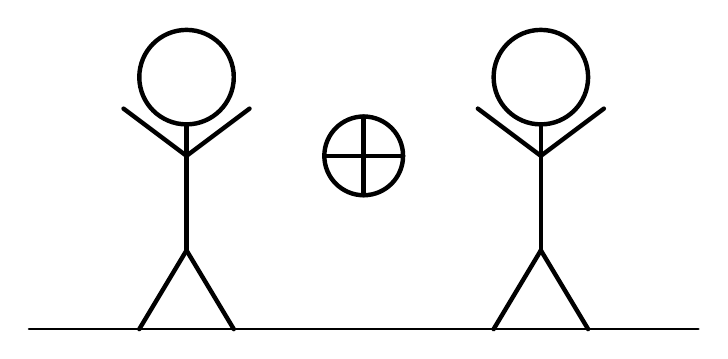
\begin{tikzpicture}[line width=1.6pt, line cap=round, line join=round]
  % niño (izquierda)
  \draw (-3,0)   circle (0.6);
  \draw (-3,-0.6) -- (-3,-2.2);
  \draw (-3,-1)  -- (-3.8,-0.4);
  \draw (-3,-1)  -- (-2.2,-0.4);
  \draw (-3,-2.2) -- (-3.6,-3.2);
  \draw (-3,-2.2) -- (-2.4,-3.2);
  % niña (derecha)
  \draw (1.5,0)  circle (0.6);
  \draw (1.5,-0.6) -- (1.5,-2.2);
  \draw (1.5,-1) -- (2.3,-0.4);
  \draw (1.5,-1) -- (0.7,-0.4);
  \draw (1.5,-2.2) -- (2.1,-3.2);
  \draw (1.5,-2.2) -- (0.9,-3.2);
  % pelota, entre los dos
  \draw (-0.75,-1) circle (0.5);
  \draw (-0.75,-1.5) -- (-0.75,-0.5);
  \draw (-1.25,-1) -- (-0.25,-1);
  % suelo
  \draw[line width=1pt] (-5,-3.2) -- (3.5,-3.2);
\end{tikzpicture}
